% !TeX spellcheck = en_GB
% ***************************************************** %
\section{Results}\label{subsc:res}
% ***************************************************** %

In order to solve the problem, we firstly explore the \emph{solution space} using the \texttt{multi-start} meta-heuristic on different TSP instances. The considered problems have different sizes: $N=\numlist{30;50}$ for circular and random layouts.\par\medskip

Exploring the solution space means to empirically find the \emph{energy landscape}, that is the distribution of each $f(x^\ast)$ of the problem. The multi-start method is applied with local search and simulated annealing as base algorithms.

We keep track of each final objective function value and each solution because two different solutions may have the same $f$ (in circular layout the circular path clockwise and counter-clockwise), so the \emph{ratio} between the number of unique local minima and starting solutions can be computed.

% TODO: increase k to 1000 and 1500?
Figure~\vref{fig:res-energy} shows these results. Increasing the number of local search iterations $k$ for a given problem instance reduces the ratio and we can see that the mode of the distribution shifts towards left, however as the problem size increases, the number of sharp local minima on which the algorithms may fall increases as well.

When the size of the problem is quite large $N=50$ the local search needs a large number of iterations, so we can increase further $k$ or move to another algorithm. However, local search will eventually fall in a local minima, but the multi-start approach can ease this situation since the local search is dependent on the starting solution and we provide a pool of $x^0$.\par\medskip

Now we can move forward to solve the problem instances with the previous methods, figure~\ref{fig:res-local-search} displays the diagnostic for the best local search obtained through the multi-start and figure~\vref{fig:res-sim-annealing} for the simulated annealing.

In both diagnostic we can see that the solutions with lower objective function value have no crossing edges. Results show that local search easily gets trapped in local minima, especially the \texttt{swap} method, while \texttt{reverse} proves to be a better choice, however both need far more iterations to reach $f(x^\ast)$ closer to simulated annealing.

In the simulated annealing diagnostic best and last accepted objective function values performance are displayed, we can see that when the acceptance rate is about $\chi(x)\approx0.5$ the $f(x^k)$ series has a negative trend and so converges with $f(x^\ast)$ while $\chi$ goes to zero, the algorithm stops when no more solution are accepted. When the problem size increases, not much the outer iterations as the length of the Markov chain needs to be increased.


\begin{figure}
\centering
\subfloat[\emph{Local search, circular layout, $\text{ratio}=\numlist{1.0;0.779}$}]%
	{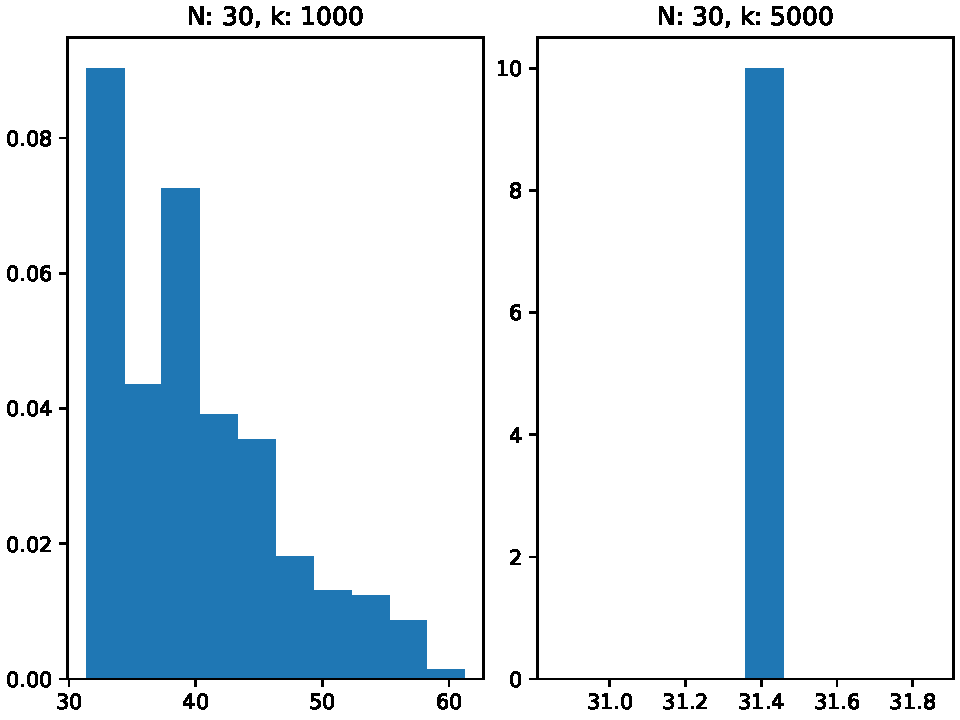
\includegraphics[width=0.49\textwidth]{circle-reverse-energy0}} \,
\subfloat[\emph{Local search, circular layout, $\text{ratio}=\numlist{1.0;1.0}$}]%
	{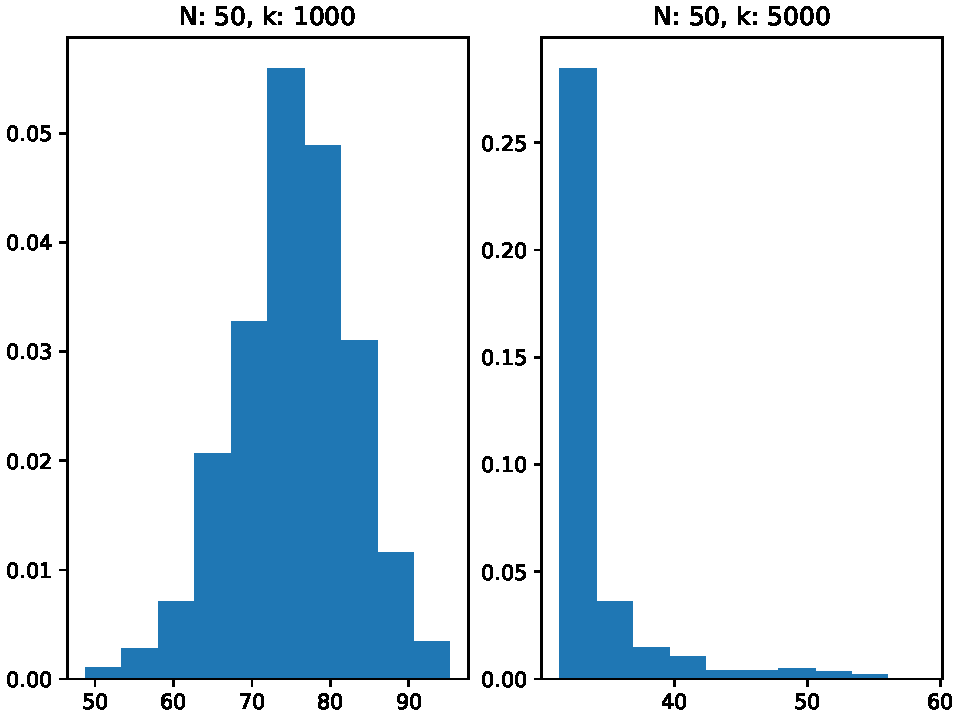
\includegraphics[width=0.49\textwidth]{circle-reverse-energy1}} \\
\subfloat[\emph{Local search, random layout, $\text{ratio}=\numlist{1.0;0.995}$}]%
	{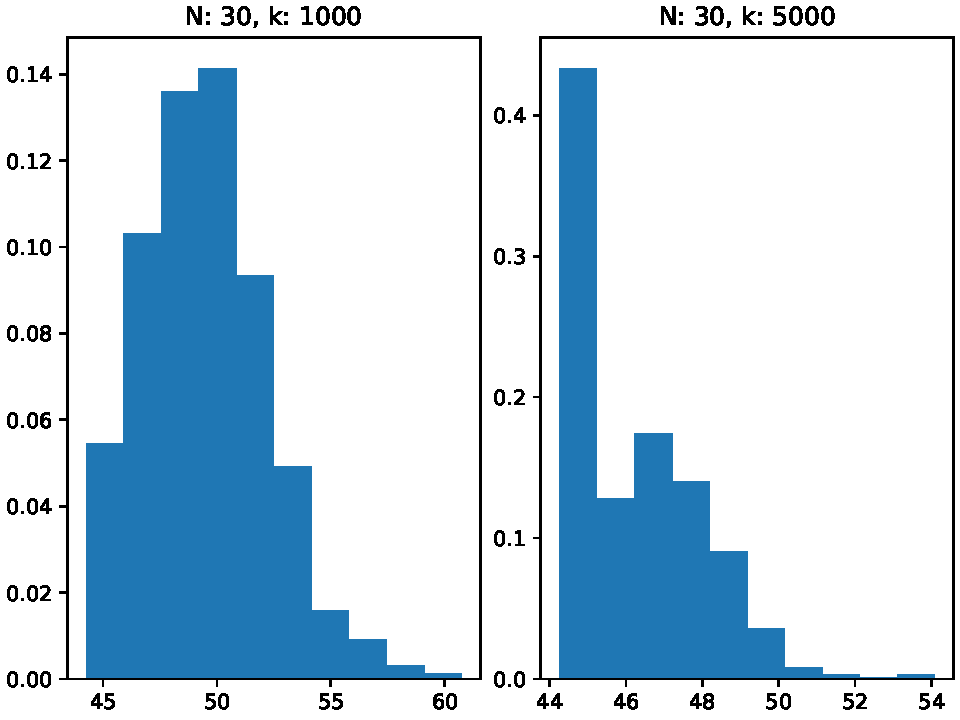
\includegraphics[width=0.49\textwidth]{rand-reverse-energy0}} \,
\subfloat[\emph{Local search, random layout, $\text{ratio}=\numlist{1.0;1.0}$}]%
	{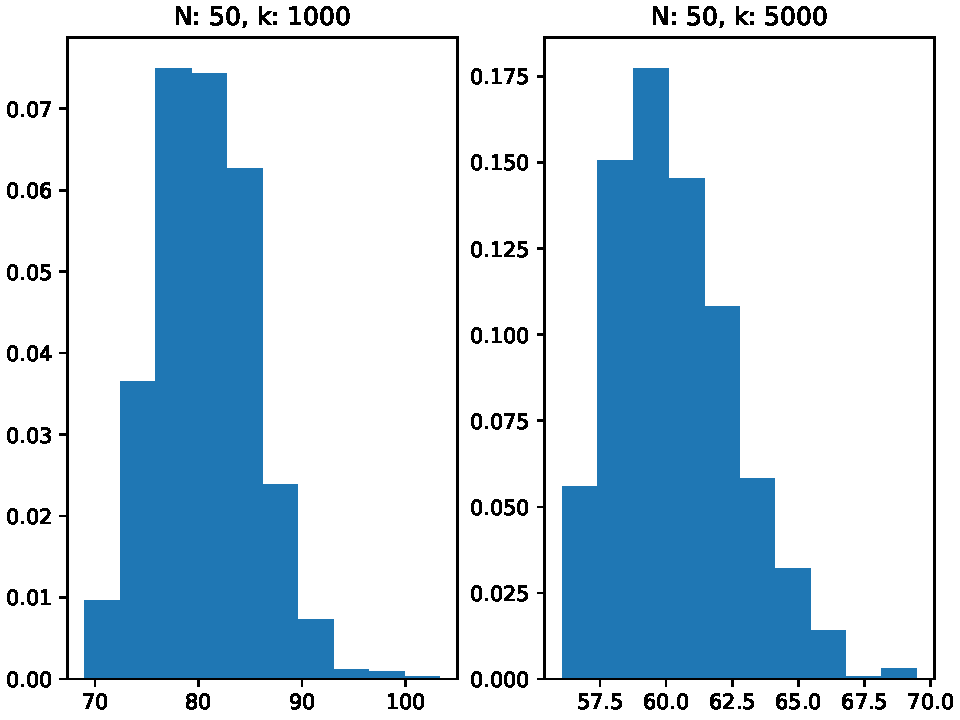
\includegraphics[width=0.49\textwidth]{rand-reverse-energy1}} \\
\subfloat[\emph{Simulated annealing, circular layout, $\text{ratio}=\numlist{0.025;0.985}$}]%
	{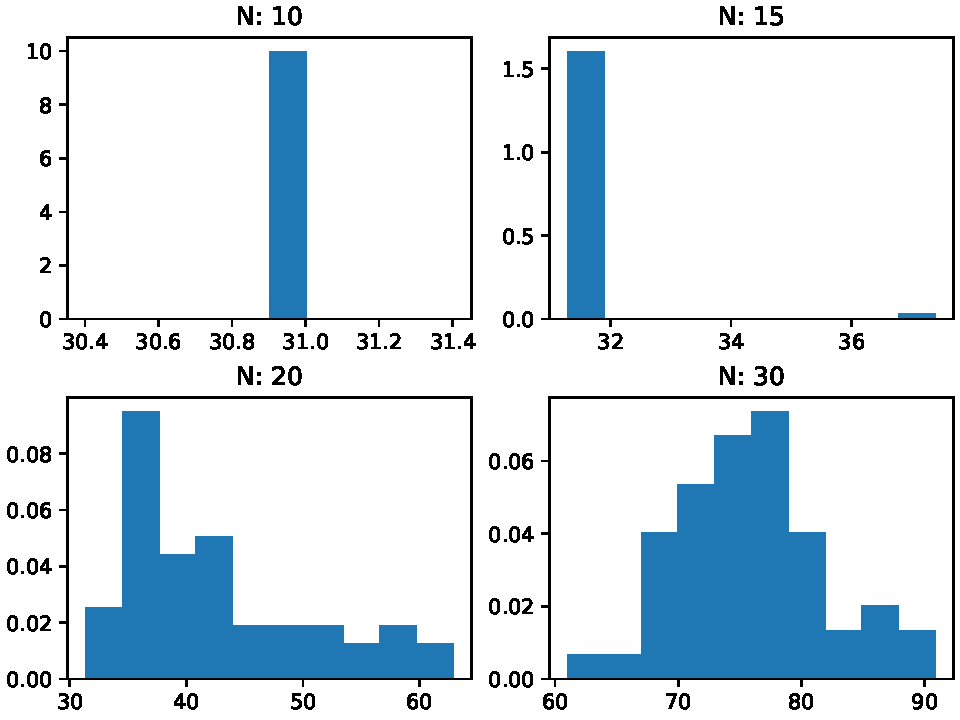
\includegraphics[width=0.49\textwidth]{circle-annealing-energy}} \,
\subfloat[\emph{Simulated annealing, random layout, $\text{ratio}=\numlist{0.465;1.0}$}]%
	{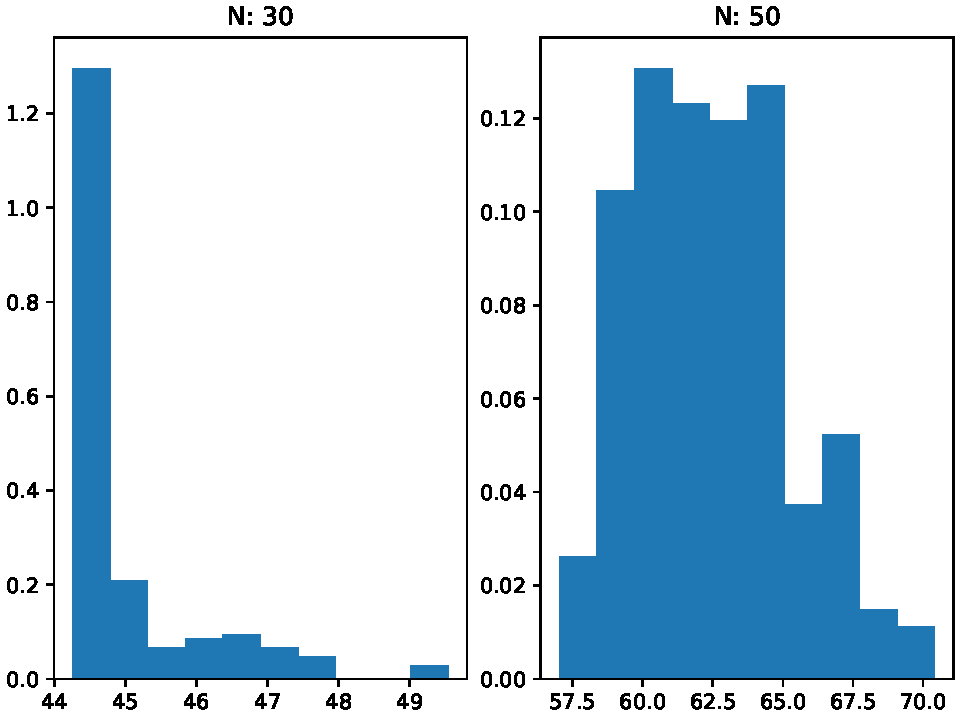
\includegraphics[width=0.49\textwidth]{rand-annealing-energy}}
\caption{Local search with \texttt{reverse} method ($k$ iterations) and SA ($k=500$, $L_k=200$, $\alpha=0.995$) energy landscapes for $N=\numlist{30;50}$ instances}
\label{fig:res-energy}
\end{figure}


\cleardoublepage\thispagestyle{empty}
\begin{figure}\vspace{-2cm}
\centering
% circular layout
\subfloat[\emph{\texttt{swap} method on circular layout}]%
	{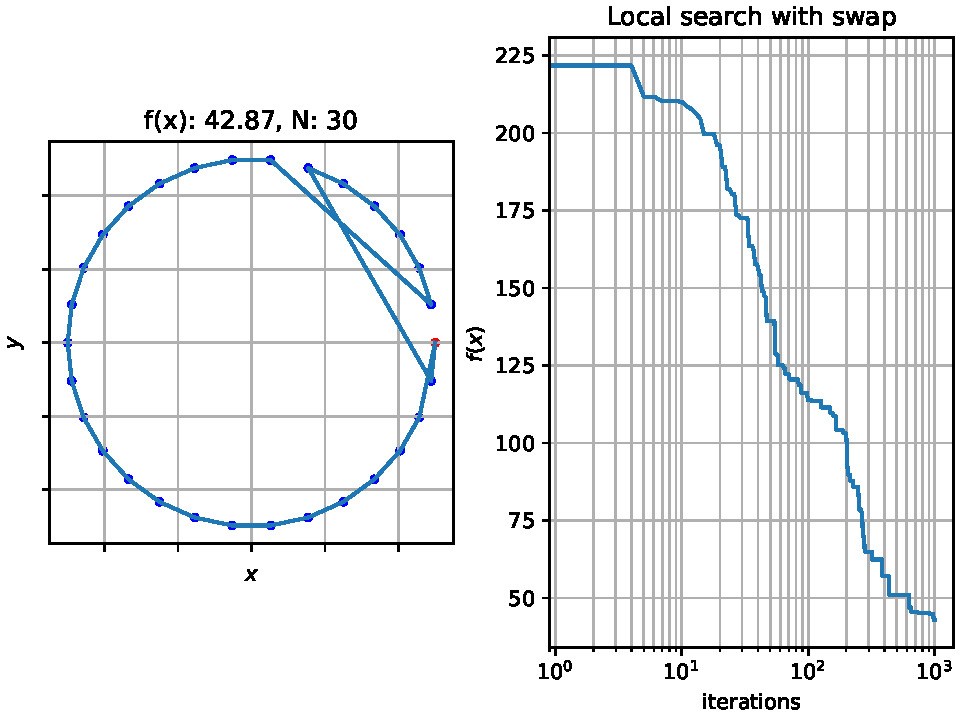
\includegraphics[width=0.49\textwidth]{circle-swap1}} \,
\subfloat[\emph{\texttt{swap} method on circular layout}]%
	{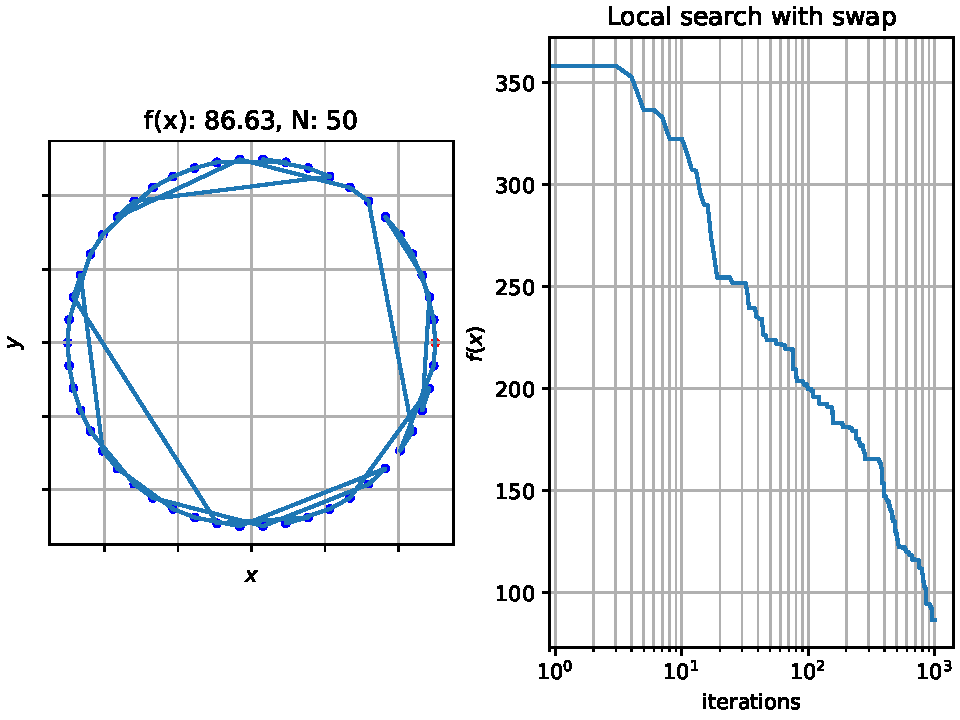
\includegraphics[width=0.49\textwidth]{circle-swap2}} \\
\subfloat[\emph{\texttt{reverse} method on circular layout}]%
	{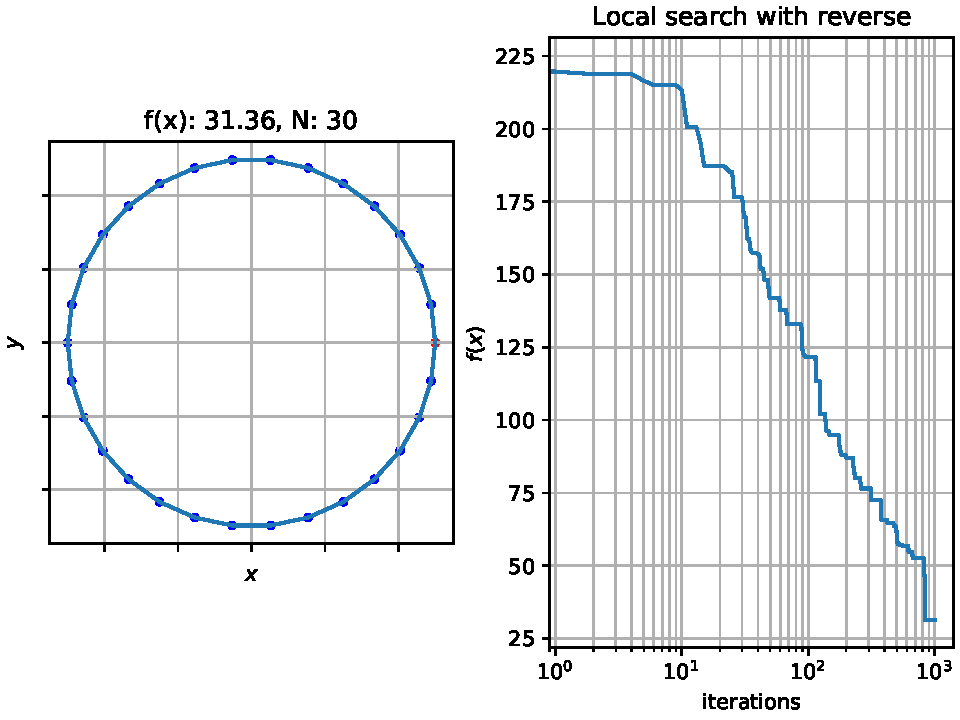
\includegraphics[width=0.49\textwidth]{circle-reverse1}} \,
\subfloat[\emph{\texttt{reverse} method on circular layout}]%
	{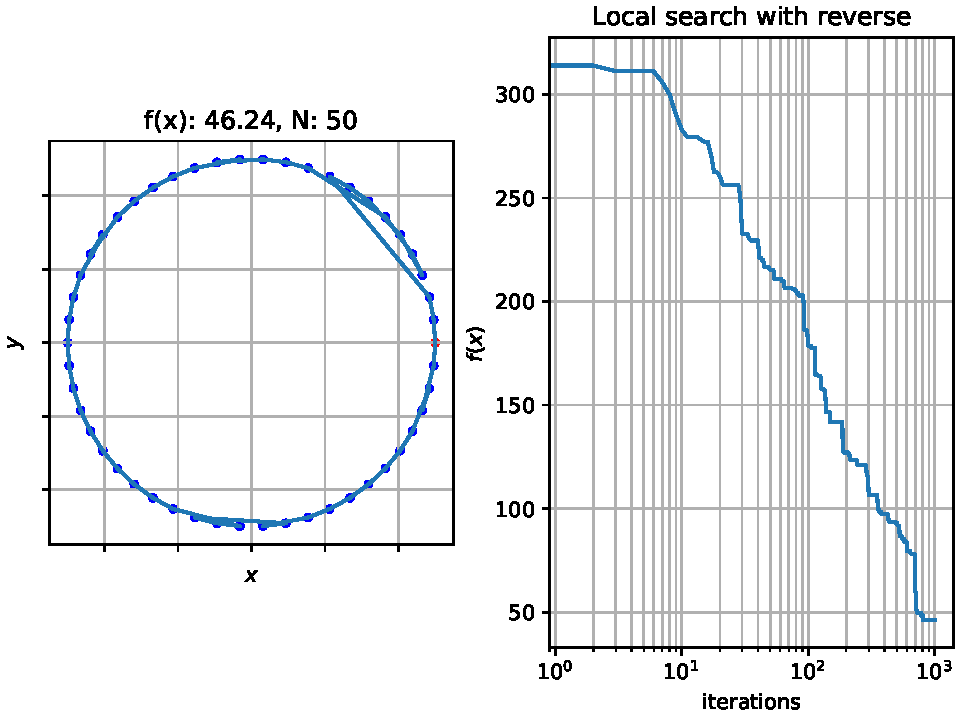
\includegraphics[width=0.49\textwidth]{circle-reverse2}} \\
% random layout
\subfloat[\emph{\texttt{swap} method on circular layout}]%
	{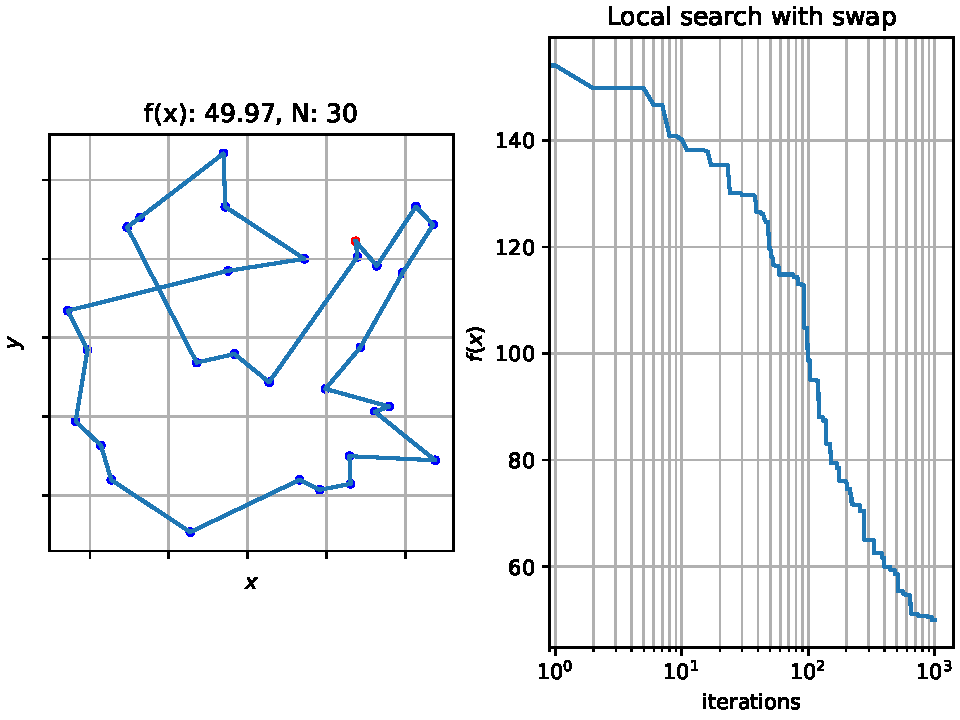
\includegraphics[width=0.49\textwidth]{rand-swap1}} \,
\subfloat[\emph{\texttt{swap} method on circular layout}]%
	{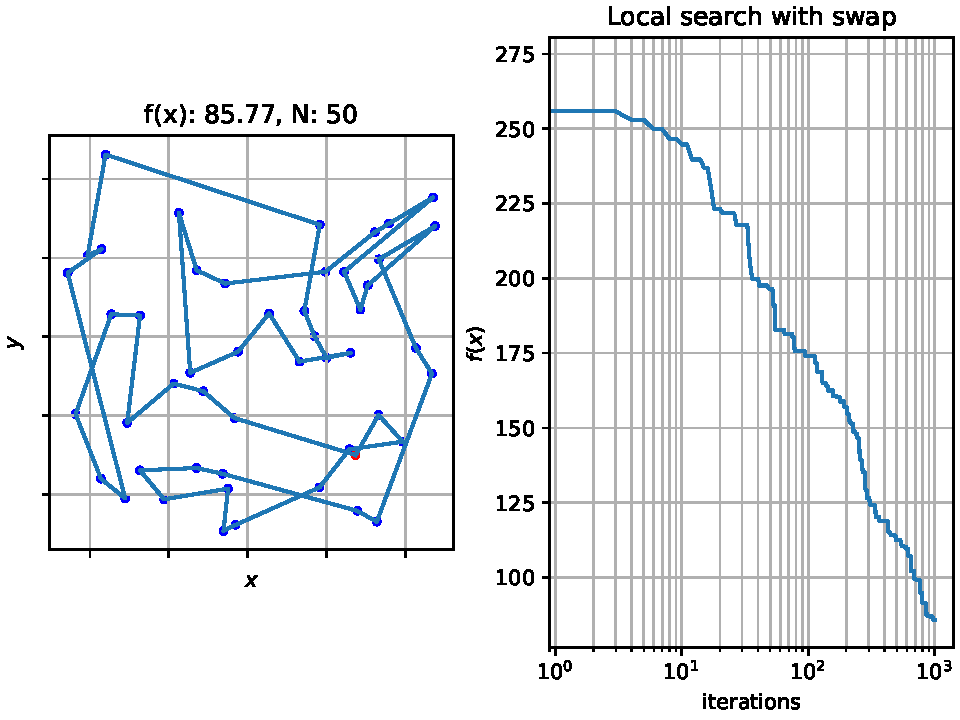
\includegraphics[width=0.49\textwidth]{rand-swap2}} \\
\subfloat[\emph{\texttt{reverse} method on circular layout}]%
	{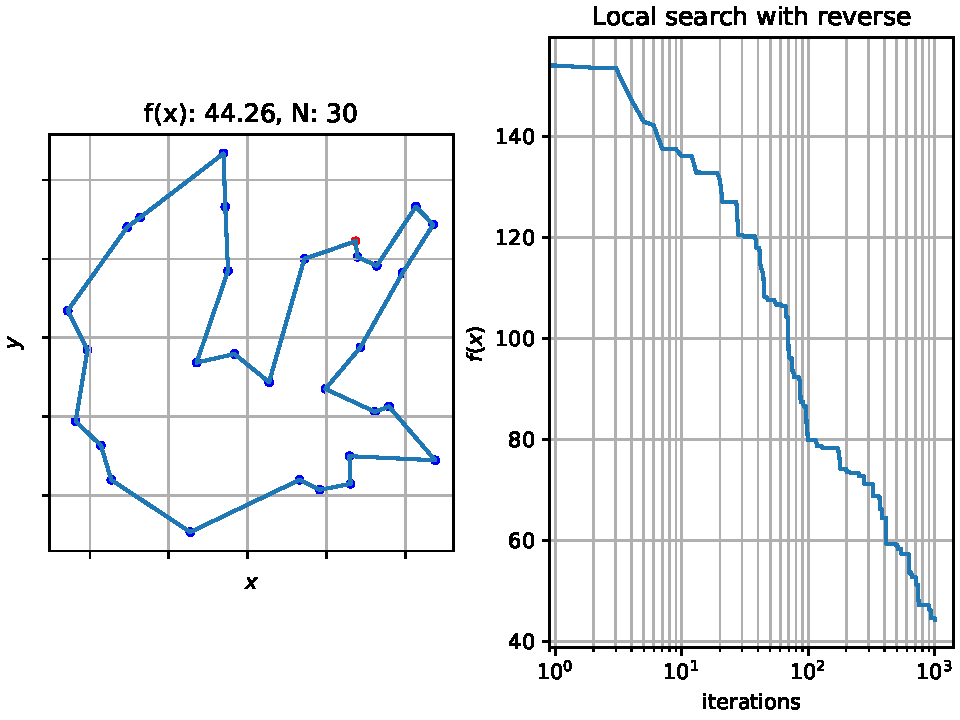
\includegraphics[width=0.49\textwidth]{rand-reverse1}} \,
\subfloat[\emph{\texttt{reverse} method on circular layout}]%
	{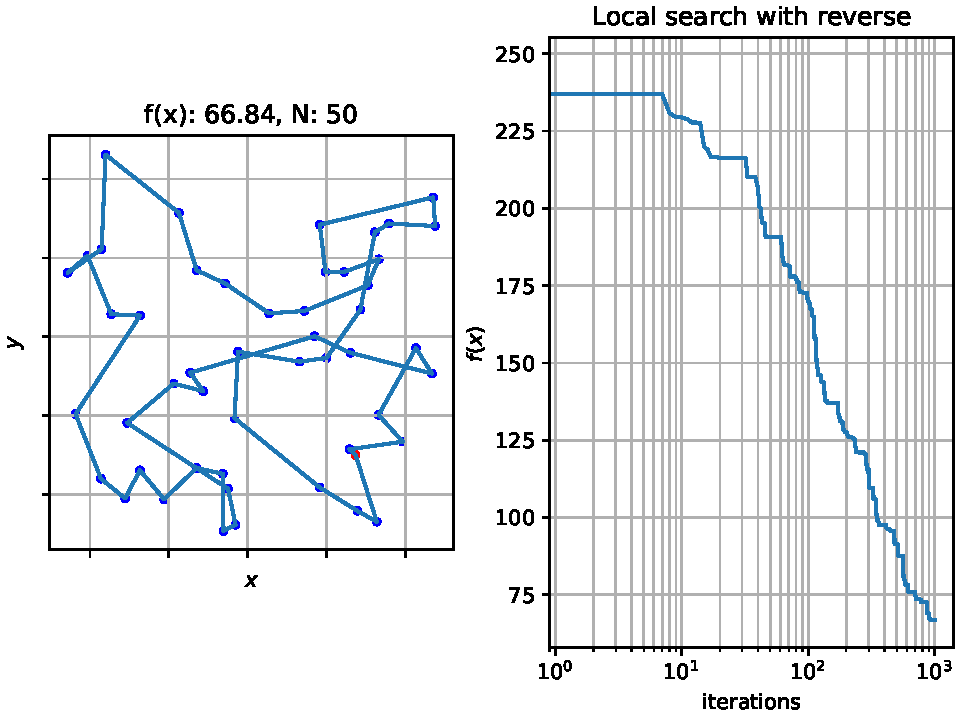
\includegraphics[width=0.49\textwidth]{rand-reverse2}}
\caption{Local search algorithms ($k=1000$) performance on problem instances. Used a multi-start procedure for selecting the best solver}
\label{fig:res-local-search}
\end{figure}
\cleardoublepage

\begin{figure}
\centering
% circular layout
\subfloat[\emph{Circular layout}]%
	{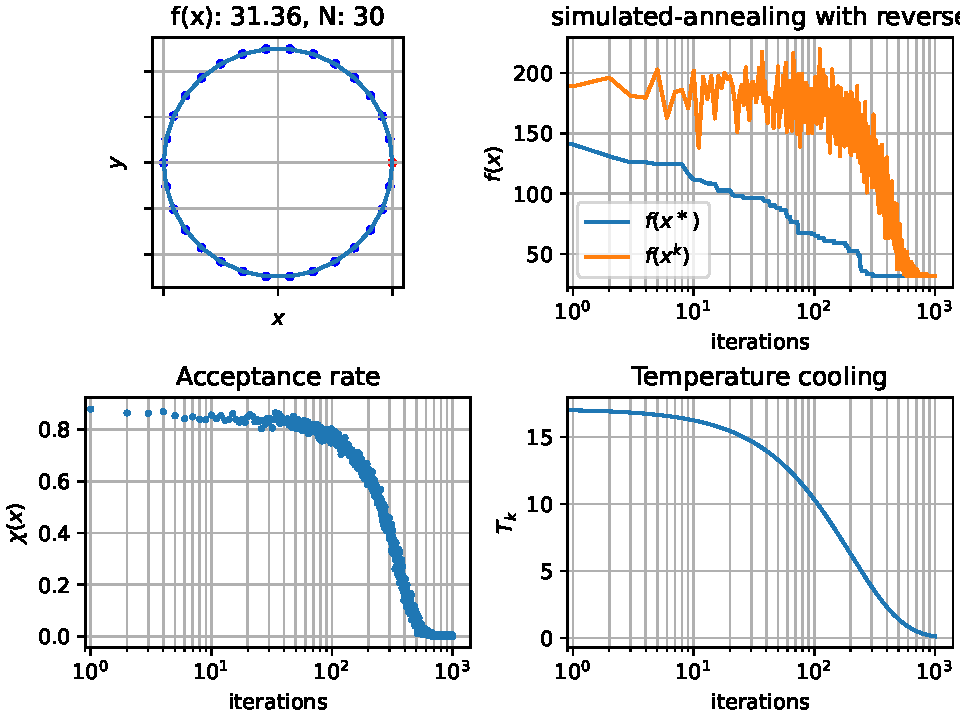
\includegraphics[width=0.49\textwidth]{circle-annealing-quad1}} \,
\subfloat[\emph{Circular layout}]%
	{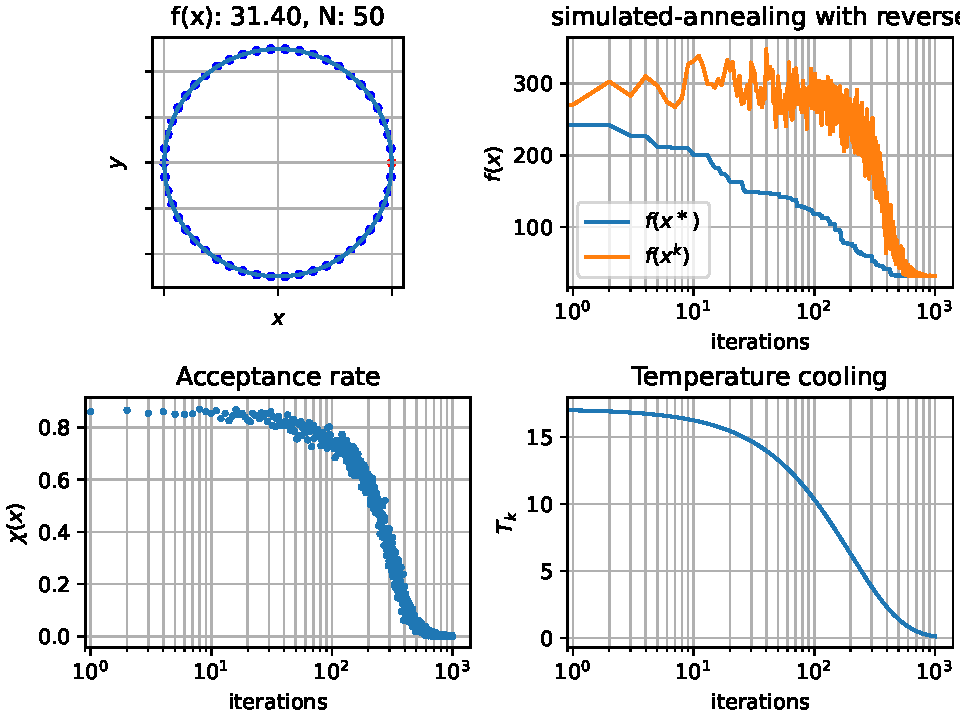
\includegraphics[width=0.49\textwidth]{circle-annealing-quad2}} \\
% random layout
\subfloat[\emph{Random layout}]%
	{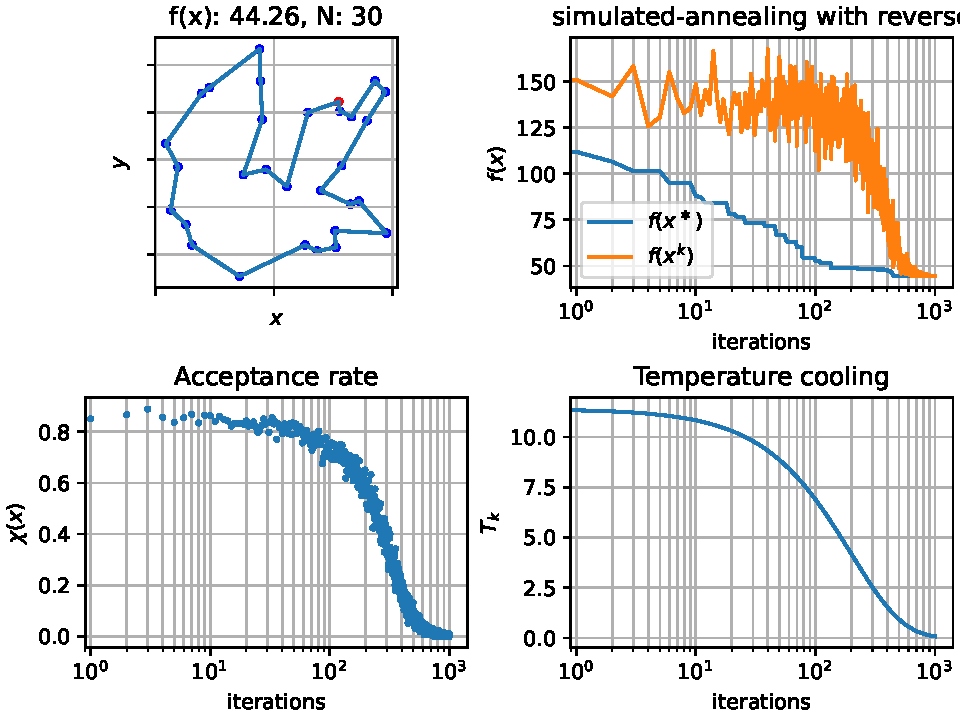
\includegraphics[width=0.49\textwidth]{rand-annealing-quad1}} \,
\subfloat[\emph{Random layout}]%
	{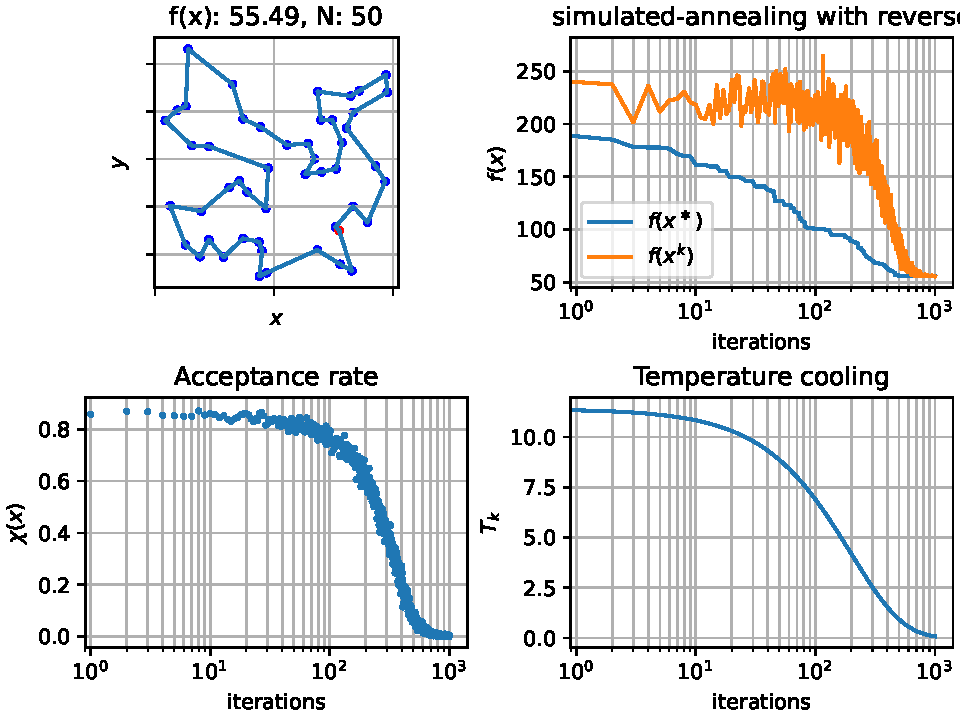
\includegraphics[width=0.49\textwidth]{rand-annealing-quad2}}
\caption{Simulated annealing ($k=1000$, $L_k=1000$, $\alpha=0.995$) performance on problem instances}
\label{fig:res-sim-annealing}
\end{figure}
